\newpage{}
\addcontentsline{toc}{section}{Обзор}
\chapter*{Обзор}
Проблему выбора структуры модели глубокого обучения можно сформулировать следующим образом: решается задача классификации или регрессии на заданной выборке. Требуется выбрать структуру нейронной сети, доставляющей минимум ошибки на этой функции и максимум качества на некотором внешнем критерии. Под моделью глубокого обучения понимается суперпозиция дифференцируемых нелинейный функций. Под структурой модели понимается значения структурных параметров модели, т.е. параметров модели, характеризующий вид итоговой суперпозиции. 


Смежной задачей к задаче выбора структуры модели является задача корректного представления структуры сети или параметризация сети глубокого обучения. Одним из возможных представлений структуры модели является графовое представление, в котором в качестве ребер графа выступают нелинейные функции, а в качестве вершин графа --- представление выборки под действием соответствующих нелинейных функций. 
Данный подход к описанию модели является достаточно общим и коррелирует с походом, описанным в~\cite{vokov}, а также в библиотеках типа TensorFlow, Caffe, Teano, Torch, в которых модель рассматривается как граф, ребрами которого выступают математические операции, а вершинами --- результат их действия на выборку. 
 В то же время, существуют и другие способы представления модели. В то же время, в ряде работ, посвященных байесовской оптимизации~\cite{snoek_deep,rbf_surrogate,bo_gp}, модель рассматривается как ``черный ящик'', имеющий ограниченный набор операций типа ``произвести оптимизацию параметров'' и ``предсказать значение зависимой переменной по независимой переменной''.
Подход, описанный в данных работах, также коррелирует с  библиотеками машинного обучения, такими как Weka, RapidMiner или sklearn, в которых модель машинного обучения рассматривается как ``черный ящик''.


Заметим, что частным случаем выбора структуры глубокой сети является выбор обобщенно-линейных моделей, т.к. отдельные слои нейросети можно рассматривать как обобщенно-линейные модели. Задачу выбора обобщенно-линейной модели можно рассматривать как задачу выбора признаков, методы решения которой делятся на три группы~\cite{feature_select}:
\begin{enumerate}
\item Фильтрационные методы. Основной особенностью данных методов является то, что такие методы не используют какой-либо информации о модели, а отсекают признаки только на основе статистических показателей. 
\item Оберточные методы --- методы, анализирующие подмножества признаков. Такие методы выбирают не признаки, а подмножества признаков, что позволяет учесть корреляция признаков.
\item Методы погружения проводят оптимизацию моделей и выбор признаков в единой процедуре, являясь комбинацией предыдущих типов отбора признаков.
\end{enumerate} 

В данном обзоре методы порождения и выбора обобщенно-линейных моделей не рассматривается в силу общности рассматриваемой задачи. 

\section{Постановка задачи}
Задана выборка  \begin{equation}\label{eq:dataset}\mathfrak{D} = \{(\mathbf{x}_i,y_i)\}, i = 1,\dots,m,\end{equation} состоящая из множества пар <<объект-метка>>, $$\mathbf{x}_i \in \mathbf{X} \subset \mathbb{R}^n, \quad {y}_i \in \mathbf{y} \subset \mathbb{Y}.$$ Метка ${y}$  объекта $\mathbf{x}$ принадлежит либо множеству: ${y} \in \mathbb{Y} = \{1, \dots, Z\}$ в случае задачи классификации, где $Z$ --- число классов, либо некоторому подмножеству вещественных чисел ${y} \in \mathbb{Y}  \subseteq \mathbb{R}$ в случае задачи регрессии.

Моделью глубокого обучения $\mathbf{f}$ назовем суперпозицию функций
\begin{equation}
\label{eq:main}
 \mathbf{f}(\mathbf{w}, \mathbf{X}) = \mathbf{f}_1(\mathbf{f}_2(\dots \mathbf{f}_K( \mathbf{X}))): \mathbb{R}^{m \times n} \to \mathbb{Y}^m,
\end{equation}
где $\mathbf{f}_k$ --- подмодели, параметрическое семейство дважды дифференцируемых по параметрам вектор-функций, $k \in \{1,\dots,K\}$; $\mathbf{w} \in \mathbb{R}^u$~---~вектор параметров моделей.\\

Для каждой модели определена функция правдоподобия  $p(\mathbf{y}|\mathbf{X}, \mathbf{w}, \mathbf{f})$, где $\mathbf{x}$ --- строка матрицы $\mathbf{X}$, $\mathbf{y}$ --- вектор меток зависимой переменной $y$.

Будем полагать, что множество рассматриваемых моделей задается некоторой функцией  $\mathfrak{F}(\beta)$. Для каждой модели $\mathbf{f}$ из конечного множества моделей $\mathfrak{F}(\beta)$ задано априорное непрерывное распределение параметров $p(\mathbf{w}|\alpha)$. 


Пусть задана дифференцируемая функция $Q$, определяющая качество модели.


\textbf{Определение }Модель классификации $\hat{\mathbf{f}}$ назовем оптимальной среди моделей $\mathfrak{F}$, если достигается максимум качества $Q$:
    $$
        \hat{\mathbf{f}}  = \arg\max_{\mathbf{f} \in \mathfrak{F}} Q(\mathbf{f}).
    $$

\textbf{Определение } Назовем оператором оптимизации алгоритм $T$ выбора вектора параметров $\mathbf{w}'$ по предыдущему значению параметров модели $\mathbf{w}$:
    $$
        \mathbf{w}' = T(\mathbf{w}, \gamma),
    $$
где $\gamma$ --- вектор параметров оптимизации.
 

Требуется найти оптимальную модель $\mathbf{f}$ среди заданного множества моделей $\mathfrak{F}$, а также значения ее параметров $\mathbf{w}$, доставляющие максимум функции $Q$:
\begin{equation}
\label{eq:main}
\mathbf{f} = \arg \min_{\mathbf{f}' \in \mathfrak{F}} \min_{\gamma, \alpha} Q,
\end{equation}
\[
\mathbf{w} = T(\mathbf{w}, \gamma).
\]

В дальнейшем будем использовать следующие наименования для групп параметров, участвующих в задаче оптимизации~\eqref{eq:main}:
\begin{enumerate}
\item $\mathbf{w}$ --- множество параметров модели.
\item $\alpha$ --- множество гиперпараметров модели.
\item $\beta$ --- множество структурных параметров.
\item $\gamma$ --- метапараметры.
\end{enumerate}


\section{Метаоптимизация}
Задача выбора структуры модели тесно связана с раздел машинного обучения под названием \textit{метаобучение}. Под метаобучением понимаются алгоритмы машинного оубчения~\cite{metalearn}, которые:
\begin{enumerate}
\item могут оценивать и сравнивать методы оптимизации моделей
\item оценивать возможные декомпозиции процесса оптимизации моделей
\item на основе полученных оценок предлагать оптимальные стратегии оптимизации моделей и отвергать неоптимальные стратегии. 
\end{enumerate}



\subsection{Теоретические основания метаобучения }
В работе~\cite{layerwise_optimal} рассматривается задача построения порождающих моделей, предлагается критерий для послойного обучения порождающих моделей:
\begin{figure}[H]
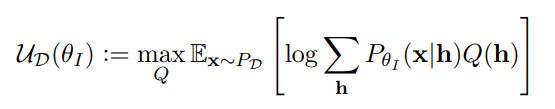
\includegraphics[width=\textwidth]{./arch_review_figs/mub.png}
\end{figure}

В работе~\cite{search_space} рассматриваются подходы к сэмплированию моделей глубокого обучения. Под \textit{сэмплированием} понимается порождение нескольких экземпляров модели из заданного распределения для дальнейшего выбора наилучшей модели. Предлагается формализация пространства поиска и формальное описание элементов  пространства моделей:
 \begin{figure}[H]
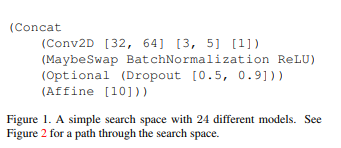
\includegraphics[width=\textwidth]{./arch_review_figs/search_space.png}
\end{figure}

\subsection{Метаоптимизация: learning to learn}
В работе~\cite{self_rnn} предлагается подход к адаптивному изменению структуры сети, основанный на обучении с подкреплением. Предлагается параметризация модели нейросети, включающая в себя модифицирующие и анализирующие выходы, позволяющие модифицировать параметры модели:
\begin{figure}[H]
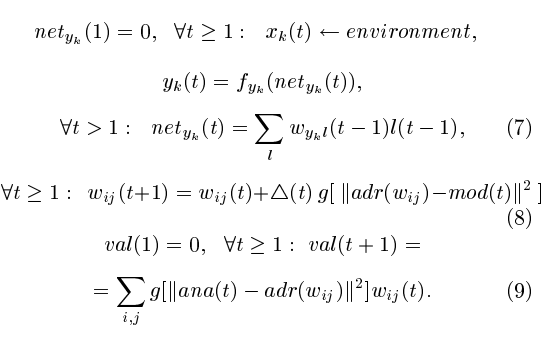
\includegraphics[width=\textwidth]{./arch_review_figs/self_rnn.png}
\end{figure}
Предлагается продолжение подхода, позволяющая рекуррентно продолжать анализ модели и порождать мета-мета-$\dots$-анализ.

В работе~\cite{meta_sgd} рассматривается оптимизация метапараметров (шага градиентного спуска и начального распределения параметров) с использованием обучения с подкреплением. На каждой итерации сэмплируется подвыборка, по которой проводится оптимизация данных метапараметров:
\begin{figure}[H]
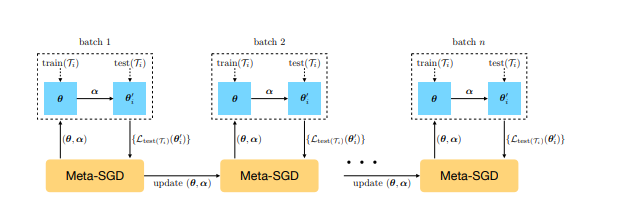
\includegraphics[width=\textwidth]{./arch_review_figs/meta_sgd.png}
\end{figure}

В работе~\cite{l2l} рассматирвается задача восстановления параметров модели по параметрам слабо обученной модели:
\begin{figure}[H]
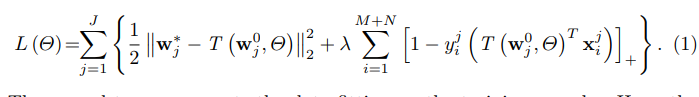
\includegraphics[width=\textwidth]{./arch_review_figs/l2l.png}
\end{figure}

\begin{figure}[H]
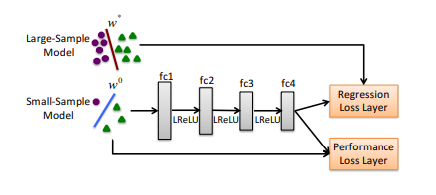
\includegraphics[width=\textwidth]{./arch_review_figs/l2l_scheme.png}
\end{figure}

В работе~\cite{l2l_by_gd_gd} рассматривается оптимизация метапараметров оптимизации с помощью LSTM, которая выступает альтернативе аналитических алгоритмов, таких как Adam или AdaGrad. LSTM имеет  (сравнительно) небольшое количество параметров, т.к. для каждого метапараметра используется своя копия модели LSTM с одинаковыми параметрами для каждой копии:
\begin{figure}[H]
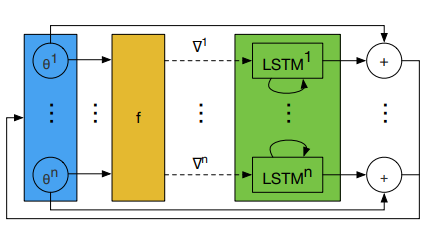
\includegraphics[width=\textwidth]{./arch_review_figs/l2lbygd.png}
\end{figure}




\subsection{Перебор структур}
В работе~\cite{search_smbo} рассматривается задача порождения сверточных нейронных сетей. Предлагается проводить поиск оптимальной структуры сети по восходящему по сложности порядку: начиная от сетей с одни блоком и наращивая блоки. В силу высокой вычислительной сложности данного подхода, вместо построения модели,предлагается обучить рекуррентную нейросеть,которая предсказывает качество модели по заданным блокам. 


В работе~\cite{optimal_racing} рассматривается задача выбора архитектуры с помощью большого количества параллельных запусков обучения моделей, предлагаются критерии ранней остановки оптимизации обучения моделей.


\subsection{ Обучение с подкреплением}
В работе~\cite{reinf} представлена схема выбора архитектуры сверточной нейросети с использованием обучения с подкреплением. В качестве актора (контроллера) выступает рекуррентная нейронная сеть.
\begin{figure}[H]
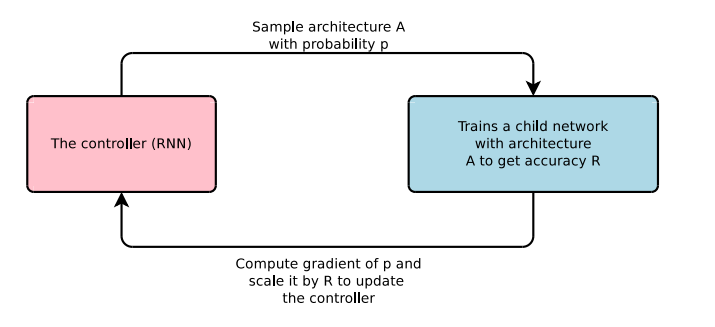
\includegraphics[width=\textwidth]{./arch_review_figs/reinf.png}
\end{figure}
В работе~\cite{reinf_predict} предлагается построение регрессионной модели для оценки финального качества модели и ранней остановки оптимизации моделей. Данный подход позволил существенно ускорить поиск моделей, представленный в работе~\cite{reinf}.
В работе~\cite{reinf_transfer} рассматривается задача переноса архитектуры нейросети, обученной на более простой выборки, на более сложную. Также предлагается параметризация пространства поиска, более делатьное, чем в~\cite{reinf}:
\begin{figure}[H]
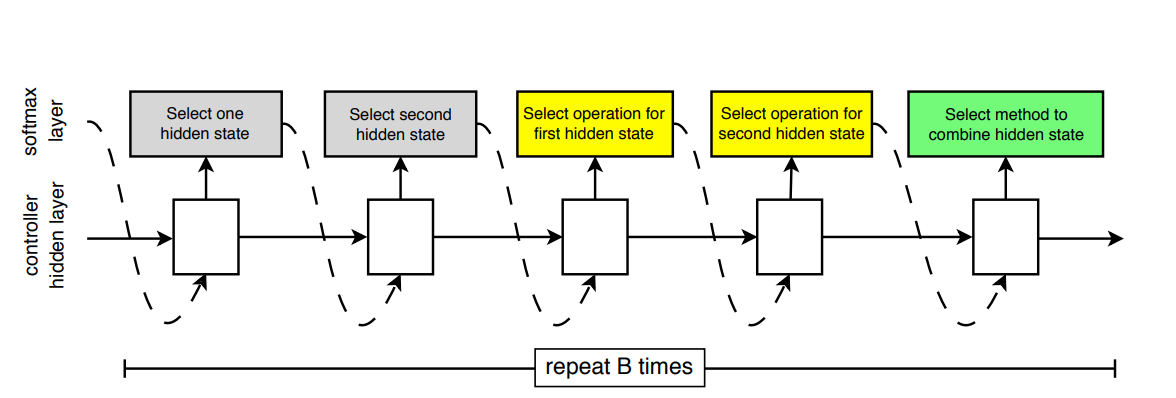
\includegraphics[width=\textwidth]{./arch_review_figs/reinf2.png}
\end{figure}

В отличие от предыдущих работ, в работе~\cite{reinf_deep2net} предлагается подход к инкрементальному обучению нейросети, основанном на модификации модели, полученной на предыдущем шаге. Рассматривается две операции над нейросетью:
\begin{itemize}
\item Расширение сети
\item Углубление сети
\end{itemize}

\begin{figure}[H]
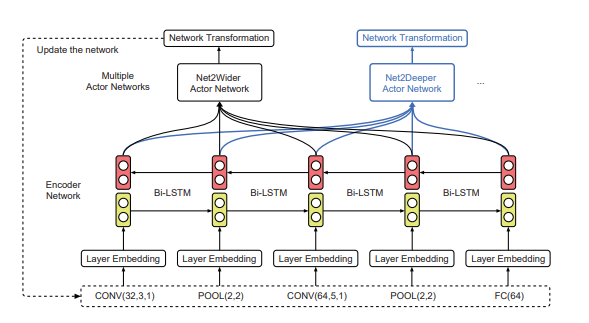
\includegraphics[width=\textwidth]{./arch_review_figs/deep2net.png}
\end{figure}



\section{Адаптивное изменение структуры}
В данном разделе собраны методы изменения структуры существующей модели. 

\textbf{Алгоритмы наращивания и прореживания параметров модели}
В работе~\cite{obd} предлагается удалять неинформативные параметры модели, где в качестве показателя информативности выступает следующий фнуционал: 
\begin{figure}[H]
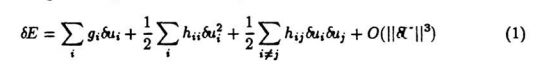
\includegraphics[width=\textwidth]{./arch_review_figs/obd.png}
\end{figure}
В работе~\cite{obs} было предложено развитие данного метода. В данной работе, в отличие от~\cite{obd} не вводится предположений о дигональности Гессиана функции ошибок, поэтому удаление неинформативных параметров модели производится точнее.

В работе~\cite{nips} был предложен метод, основанный на получении вариационной нижней оценки правдоподобия модели. В качестве критерия информативности параметра выступало отношение вероятности нахождения параметра в пределах априорного распределения к вероятности равенста параметра нулю:
\begin{figure}[H]
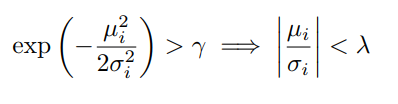
\includegraphics[width=\textwidth]{./arch_review_figs/nips_var.png}
\end{figure}
Идея данного метода была развита в~\cite{bayes_compr}, где также используются вариационные методы. В отличие от предыдущей работы, в данной работе рассматривается ряд априорных распределений параметров, позволяющих прореживать модели более эффективно:
\begin{itemize}
\item Нормальное распределение с лог-равномерным распределением дисперсии, независимой для каждого нейрона:
\begin{figure}[H]
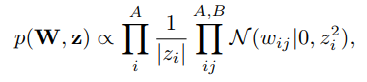
\includegraphics[width=\textwidth]{./arch_review_figs/bayes_compr_group.png}
\end{figure}
\item Произвденеие двух половинных распределений Коши: одно ответственно за отдельный параметр, другое --- за общее распределение параметров:
\begin{figure}[H]
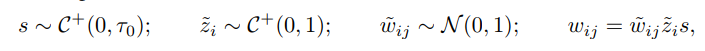
\includegraphics[width=\textwidth]{./arch_review_figs/bayes_compr_cauchy.png}
\end{figure}
\end{itemize}

Смежной темой к прореижванию моделей выступает компрессия нейросетей. Основным отличием задачи прореживания и компрессии выступает эксплуатационное требование: если прореживание используется для получения оптимальной и наиболее устойчивой модели, то компрессия часто производится для сохранения памяти и основных эксплуатационных характеристик исходной модели (?).
В работе~\cite{nvidia_prune}
предлагается итеритавиное использование регуляризации типа DropOut~\cite{dropout} для прореживания модели. 
В работах~\cite{weight_quantization, weight_quantization2} используются методы снижения вычислительной точности представления парамеров модели на основе кластеризации весов.
В работе~\cite{weight_quantization2} предлагается метод компрессии, основанный на кластеризации значений параметров модели и представлении их в сжатом виде на основе кодов Хаффмана.

В работах~\cite{boost_res, adanet} предлагается наращивание моделей, основанное на бустинге. В работе рассматривается задача построения нейросетевых моделей специального типа:
\[
    f_{t+1} = \sigma(f_t) + f_t,
\]
приводится параметризация модели, позволяющая рассматривать декомпозировать модель на слабые классификаторы.
В работе~\cite{adanet} на каждом шаге построения выбирается одно из двух расширений модели, каждое из которых рассматирвается как слабый классификатор:
1. Сделать модель шире
2. Сделать модель глубже
\begin{figure}[H]
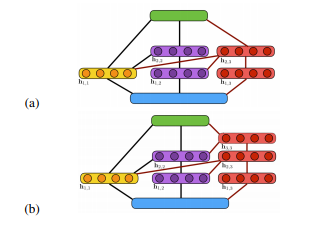
\includegraphics[width=0.5\textwidth]{./arch_review_figs/adanet.png}
\end{figure}
Построение модели заканчивается при условии снижении радемахереовской сложности:
\begin{figure}[H]
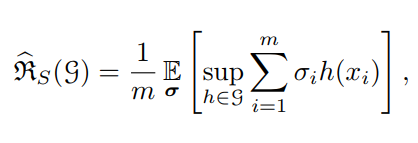
\includegraphics[width=0.5\textwidth]{./arch_review_figs/rad.png}
\end{figure}



\section{Байесовские методы порождения и выбора моделей}
\subsection{Автоматическое определение релевантности параметров}
В работе~\cite{hyper} рассматривается задача оптимизации гиперпараметров.  Авторы предлагают оптимизировать константы $l_2$-регуляризации отдельно для каждого параметра модели, проводится параллель с методами автоматического определения релевантности параметров (ARD)~\cite{MacKay}.

В работе~\cite{ard} рассматривается метод ARD для снижения размерности скрытого пространства вариационных порождающих моделей: скрытая переменная параметризуется как  произведение некоторой случайной величины $\mathbf{z}$  на вектор, отвечающий за релевантность каждой компоненты скрытой переменной:
\begin{figure}[H]
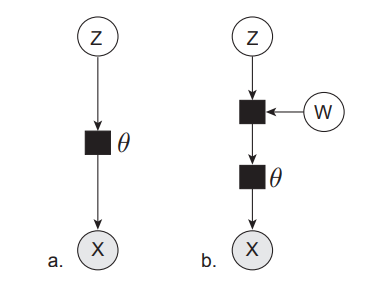
\includegraphics[width=0.5\textwidth]{./arch_review_figs/ard.png}
\end{figure}

\subsection{Суррогаты}
В работе~\cite{bo_gp} предлагается моделировать качество модели гауссовым процессом, параметрами которого выступают гиперпараметры исходной модели.
Модель, аппроксимирующая качество исходной модели, называется суррогатом. 

Одна из основных проблем использования гауссового процесса как суррогатной модели --- кубическая сложность оптимизации. В работе~\cite{random_gaus} предлагается использовать случайные подпространства гиперпараметров для ускоренной оптимизации.  В работе~\cite{gp_tree} предлагается кобминация из множества гауссовых моделей и линейной модели, позволяющая модели нелинейные зависимости гиперпараметров, а также существенно сократить сложность оптимизации. 

В работе~\cite{rbf_surrogate} предлагается рассматривать RBF-модель для аппроксимации качества исходной модели, что позволяет ускорить процесс оптимизации суррогатной модели. В~\cite{snoek_deep} рассматривается глубокая нейронная сеть в качестве суррогатной функции. Вместо интеграла правдоподобия, который оценивается в случае использования гауссового процесса в качестве суррогата, используется максимум апостериорной веротяности.

Важным параметром гауссовых процессов является функиия ядра гауссового процесса, полностью определяющая процесс в случае нулевого среднего. В работе~\cite{gp_fusion} предлагается функция ядра, определенная на графах:
    \[
    k(x,y) = r(d(x,y)),
    \]
где $d$ --- геодезическое расстояние между вершинами графа, $r$ --- некоторая вещественная функция (наверно положительно определенная, но это не указано явно в статье).
В работе~\cite{gp_arc} рассматривается задач выбора структуры нейросети, предлагается ядро специального вида, позволюящее учитывать только те гиперпапараметры, которые есть в обеих сравниваемых моделях: к примеру, для двуслойной и трехслойной нейросети будут уччитываться гиперпараметры, отвечающие только за первые два слоя. 
\begin{figure}[H]
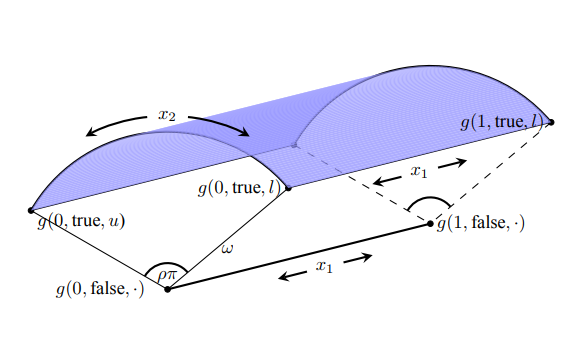
\includegraphics[width=0.5\textwidth]{./arch_review_figs/arc.png}
\end{figure}


\subsection{Адаптивное изменение структуры}

В работе~\cite{cib} рассматривается порождение unsupervised-моделей с использованием расширения процесса Индийского Буфета:
\begin{figure}[H]
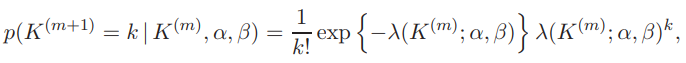
\includegraphics[width=0.5\textwidth]{./arch_review_figs/cib_eq.png}
\end{figure}
\begin{figure}[H]
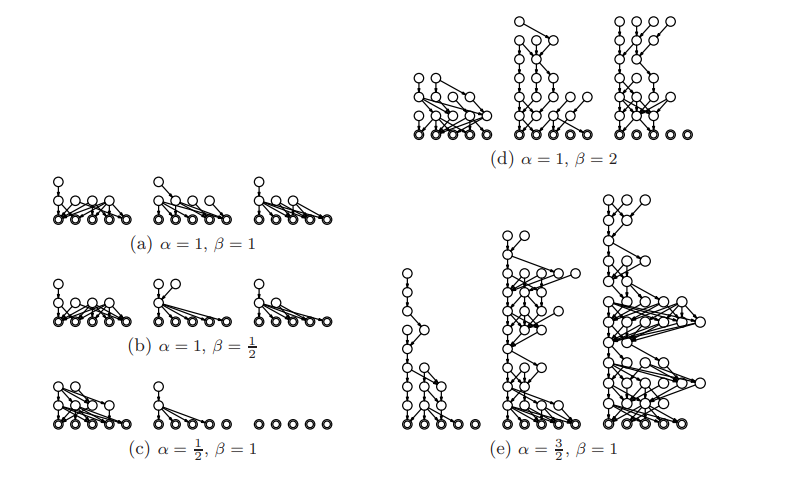
\includegraphics[width=0.5\textwidth]{./arch_review_figs/cib.png}
\end{figure}

В работе~\cite{cib_simple} предлагается упрощенная модель Индийского Буфета:
\begin{figure}[H]
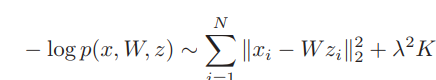
\includegraphics[width=0.5\textwidth]{./arch_review_figs/cib_simple.png}
\end{figure}

В работе~\cite{shirakawa2018dynamic} предлагается параметризация структуры модели с использованием Бернуллиевских величин:
каждая величина отвечает за включение или выключение слоя сети.



\subsection{Порождающие модели}
В работе~\cite{Kingma} было предложено обобщение вариационного автокодировщика на случай частичного обучения: 
итоговая модель вариационного автокодировщика является порождающей моделью, учитывающий метки объектов. 

В работе~\cite{vae_graph} рассматривается обобщение вариационного автокодировщика на случай более общих графических моделей. Рассматривается проводить оптимизацию сложных графических моделей в единой процедуре. Для вывода предлагается использовать нейронные сети.
Другая модификация вариационного автокодировщика представлена в работе~\cite{vae_stick}, авторы рассматривают использование процесса сломанной трости в вариационном автокодировщике, тем самым получая модель со стохастической размерностью скрытой переменной. В работе~\cite{vae_mix} рассматривается смесь автокодировщиков, где смесь моделируется процессом Дирихле.


В работе~\cite{var_boost} предлагается подход к оптимизации неизвестного распределения с помощью вариационного вывода. Авторы предлагают решать задачу оптимизации итеративно, добавляя в модель новые компоненты вариационного распределения, проводится аналогия с бустингом.
\subsection{Состязательные модели}

\section{Способы прогнозирования графовых структур}
В разделе собраны ключевые работы по порождению графовых моделей.

В работе~\cite{jaakkola2010learning} предлагается метод прогнозирования графовой структуры на основе линейного программирования. Предлагается свести проблему поиска графовой структуры к комбинаторной проблеме.

В работе~\cite{double_rnn} предлагается метод прогнозирования структур деревьев, основанный на дважды-рекуррентных нейросетях (doubly-reccurent), т.е. на сетях, отдельно предсказывающих глубину и ширину уровней деревьев.
\begin{figure}[H]
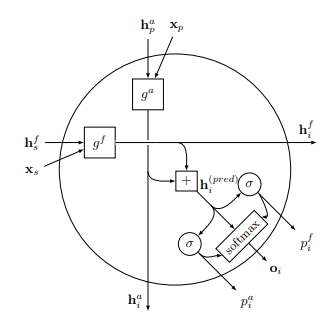
\includegraphics[width=0.5\textwidth]{./arch_review_figs/jaakkola.png}
\end{figure}


\section{Эвристические и прикладные методы}
\subsection{Эвристические методы}
В работе~\cite{layer_probe} предлагается метод анализа структуры сети на основе линейных классификаторов, построенных на промежуточных слоях нейросети.
Схожий метод был предложен в~\cite{branches}, где классификаторы на промежуточных уровнях используются для уменьшения вычислений при выполнении вывода и предсказаний.
Промежуточные классификаторы.работают как решающий список
http://www.eecs.harvard.edu/~htk/publication/2016-icpr-teerapittayanon-mcdanel-kung.pdf

В работе~\cite{nn_inc} предлагается инкрементальный метод построения нейросети: на каждом этапе построения в модель добавляются новые слои. Для улучшения качества модели, слои добавляются в начало модели, и затем проходят оптимизацию.

\subsection{Структуры сетей специального вида}
В данном разделе представлены работы по поиску оптимальной структуры сети, описывающие частные случаи поиска оптимальных моделей со структурами специального вида.

В работе~\cite{mixed} рассматривается оптимизация моделей нейросетей с бинарной функцией активацией. Задача оптимизации сводится к задаче mixed integer программирования, которая решается методами выпуклого анализа.


SKIP-сети, нужно ли писать? ResNet?
%https://papers.nips.cc/paper/6205-swapout-learning-an-ensemble-of-deep-architectures.pdf
%https://arxiv.org/pdf/1603.09382.pdf

%https://arxiv.org/pdf/1711.03130.pdf
В работе~\cite{energynet} предлагается метод построения сети глубокого обучения, структура которой выбирается с использованием обучения без учителя. Критерий оптимальности модели использует оценки энергитических функций и ограниченной машины Больцмана.

%https://arxiv.org/pdf/1511.02954.pdf
%https://arxiv.org/pdf/1701.08734.pdf
В работах~\cite{pathnet, supernet} рассматривается выбор архитектуры сети с использованием \textit{суперсетей}: больших связанных между собой сетей, образующих граф, пути в котором определяют итоговую архитектуру нейросети. В работе~\cite{supernet} рассматриваются стохастические суперсет, позволяющие выбрать структуру нейросети за органиченное время оптимизации. 
Схожий подход был предложен в работе~\cite{pathnet}, где предлагается использовать эволюционные алгоритмы для запоминания оптимальных подмоделей и переноса этих моделей в другие задачи.
\begin{figure}[H]
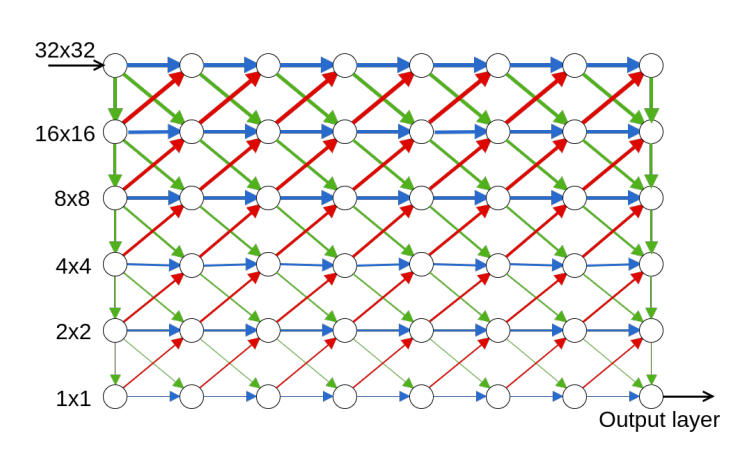
\includegraphics[width=0.5\textwidth]{./arch_review_figs/supernets.png}
\end{figure}

%https://arxiv.org/pdf/1511.02954.pdf 
%https://arxiv.org/pdf/1511.05641.pdf
%https://arxiv.org/pdf/1701.03281.pdf
В работах~\cite{net2net, morph, partition} рассматриваются методы деформации нейросетей. 
В работе~\cite{partition} предлагается метод оптимального разделения нейросети на несколько независимых сетей для уменьшения количества связей и, как следствие, уменьшения сложности оптимизации модели. В работе~\cite{net2net} предлагается метод сохранения результатов оптимизации нейросети при построении новой более глубокой или широкой нейросети. 
В работе~\cite{morph} рассматривается задача расширения сверточной нейросети, нейросеть рассматривается как граф.




